\subsection{Part 1}

The following figure shows the block diagram of traffic flows/overflows within
the system. The A values ($A_{micA}$, $A_{micB}$, $A_{micC}$, $A_{mac}$, represent the
``Offered Load'' to the cells (Micro Cell A, Micro Cell B, Micro Cell C, Macro
Cell) respectively. $N_{mic}$ represents the number of channels in the micro
cells, while  $N_{mac}$ represents the number of channels in the macro cell. The
``Offered Load'' for the Overflow is represented by $A^*$, with the number of
channels represented by $N_{mac} + N^*$.

\begin{figure}[H]
	\centering
	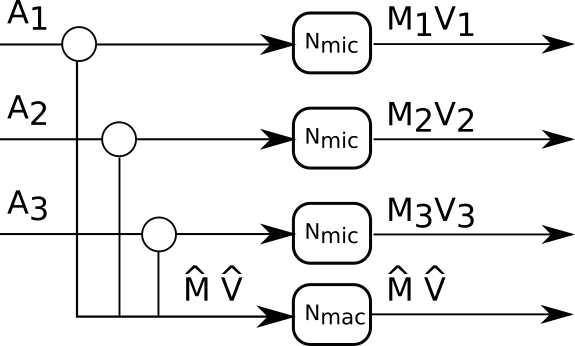
\includegraphics[width=0.8\textwidth]{images/Q6}
	\caption{Traffic Flows/Overflows Block Diagram}
	\label{fig:images-Q6}
\end{figure}
